\documentclass[a4paper,hidelinks,12pt]{article}
\usepackage[T2A]{fontenc}
\usepackage[utf8]{inputenc}
\usepackage[russian]{babel}
\usepackage{amsmath,graphicx}
\usepackage{indentfirst}
\usepackage{colortbl}
\usepackage{setspace}
\usepackage{float}
\usepackage{amssymb}
\usepackage{amsmath}
\usepackage{graphicx}
\usepackage{listings}
\usepackage{subcaption}
\usepackage{xcolor}
\usepackage{algorithm}
\usepackage{algpseudocode}
\usepackage{tabularx}
\usepackage{pdfpages}
\usepackage{array}      % для настройки столбцов
\usepackage{booktabs}   % для красивых линий
\usepackage{multirow}
\usepackage{makecell}   % для \makecell
\usepackage{graphicx}
\usepackage{adjustbox}
\usepackage{enumitem}
\RequirePackage{booktabs}
\definecolor{gray}{rgb}{0.4,0.4,0.4}
\definecolor{darkblue}{rgb}{0.0,0.0,0.6}
\definecolor{cyan}{rgb}{0.0,0.5,0.5}
\definecolor{maroon}{rgb}{0.5,0,0}
\definecolor{darkgreen}{rgb}{0,0.5,0}


\usepackage[left=3cm,right=1.5cm,top=2cm,bottom=2cm,bindingoffset=0cm]{geometry}
\setcounter{secnumdepth}{4}
\linespread{1.5}
\usepackage{xcolor}

\newenvironment{alphasection}{%
	\ifnum\alphainsection=1%
	\errhelp={Let other blocks end at the beginning of the next block.}
	\errmessage{Nested Alpha section not allowed}
	\fi%
	\setcounter{alphasect}{0}
	\def\alphainsection{1}
}{%
	\setcounter{alphasect}{0}
	\def\alphainsection{0}
}%

% \begin{document}
% \fixmargins
% \makepreliminarypages

% \oneandhalfspace

% \tableofcontents

% \section{Введение}
\label{sec:Chapter0} \index{Chapter0}

\todo[inline]{В этой части надо описать предметную область, задачу из которой вы будете решать, объяснить её актуальность (почему надо что-то делать сейчас?).
Здесь же стоит ввести определения понятий, которые вам понадобятся в постановке задачи.}


 % Введение
% \section{Постановка задачи}
\label{sec:Chapter1} \index{Chapter1}
\todo[inline]{Здесь надо максимально формально описать суть задачи, которую потребуется решить, так, чтобы можно было потом понять, в какой степени полученное в результате работы решение ей соответствует. Текст главы должен быть написан в стиле технического задания, т.е. содержать как описание задачи, так и некоторый набор требований к решению} % Постановка задачи
% \section{Обзор существующих решений}
\label{sec:Chapter2} \index{Chapter2}
\todo[inline]{Здесь надо рассмотреть все существующие решения поставленной задачи, но не просто пересказать, в чем там дело, а оценить степень их соответствия тем ограничениям, которые были сформулированы в постановке задачи.} % Обзор существующих решений
% \section{Исследование и построение решения задачи}
\label{sec:Chapter3} \index{Chapter3}
\todo[inline]{Здесь надо декомпозировать большую задачу из постановки на подзадачи и продолжать этот процесс, пока подзадачи не станут достаточно простыми, чтобы их можно было бы решить напрямую (например, поставив какой-то эксперимент или доказав теорему) или найти готовое решение.} % Исследование и построение решения задачи
% \section{Описание практической части}
\label{sec:Chapter4} \index{Chapter4}
\todo[inline]{Если в рамках работы писался какой-то код, здесь должно быть его описание: выбранный язык и библиотеки и мотивы выбора, архитектура, схема функционирования, теоретическая сложность алгоритма, характеристики функционирования (скорость/память).} % Описание Экспериментальной части
% \section{Заключение}
\label{sec:Chapter5} \index{Chapter5}
\todo[inline]{Здесь надо перечислить все результаты, полученные в ходе работы. Из текста должно быть понятно, в какой мере решена поставленная задача.} % Заключение

% \nocite{*}
% \bibliographystyle{gost71u} % Для соответствия требованиям об оформлении списка литературы
% \bibliography{references}

% % \section*{Приложение}
\addcontentsline{toc}{section}{Приложение}
\label{sec:Apendix} \index{Apendix}

 

% \end{document}

\begin {document}
\begin {titlepage}
\thispagestyle{empty}

\begin{center}
	\vspace{-1cm}
	
	
	%
	% No necessity to specify laboratory.
	%
	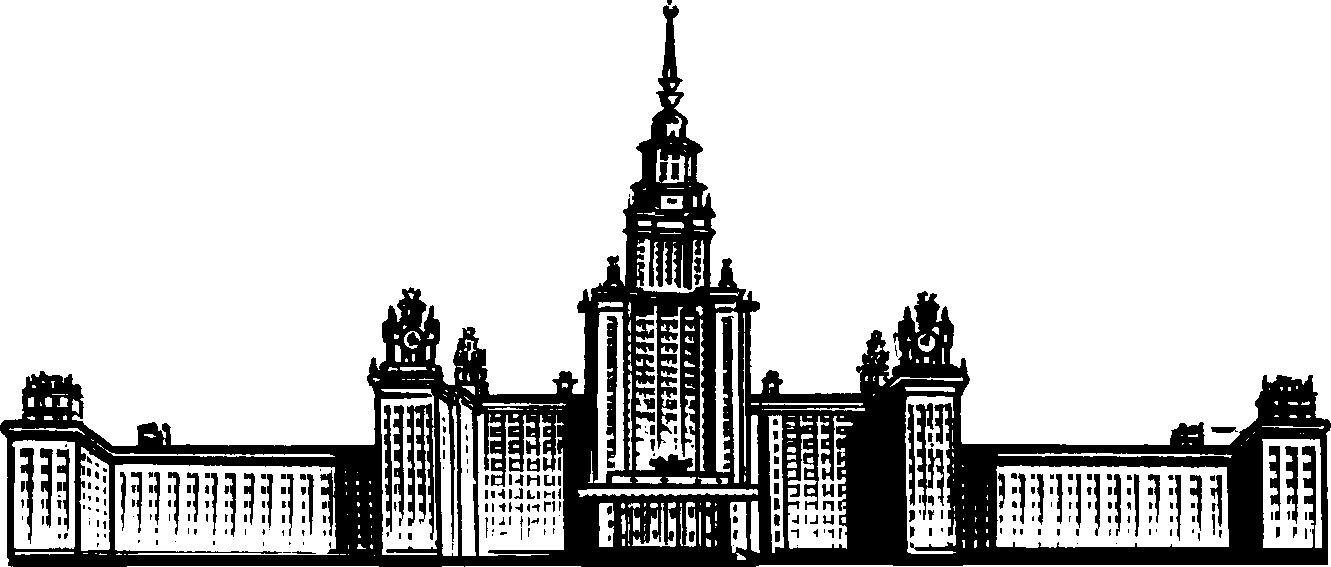
\includegraphics[width=0.5\textwidth]{gzlogo.png}\\
	Московский Государственный Университет им. М.В. Ломоносова\\
	Факультет Вычислительной Математики и Кибернетики\\
	Кафедра Интеллектуальных Информационных Технологий\\
	
	\vspace{3cm}
	
	{\Large Никитин Сергей Денисович}
	
	\vspace{1cm}
	
	{\LARGE\bfseries Сравнительный анализ представлений функций дистанции со знаком\\}
	
	\vspace{1cm}
	
	{ ВЫПУСКНАЯ КВАЛИФИКАЦИОННАЯ РАБОТА}
\end{center}

\vfill

\begin{flushright}
	\textbf {Научный руководитель:}\\
	к.ф.-м.н.\\
	В.А.Фролов\\
	\vspace{10mm}
\end{flushright}

\vfill

\begin{center}
	Москва, 2025
\end{center}

\end{titlepage}

\setcounter{page}{2}
\onehalfspacing

\begin{abstract}
	Дипломная работа посвящена сравнительному анализу функций дистанции со знаком (SDF) в 
	задачах рендеринга 3D-моделей. Целью исследования является разработка и реализация бенчмарка для оценки различных 
	представлений SDF по метрикам качества изображения (PSNR), времени рендеринга и размера модели. В работе 
	рассмотрены теоретические основы SDF, включая аналитические, воксельные и нейронные представления, а также 
	проведён обзор существующих подходов и их ограничений. Разработанный бенчмарк позволяет рендерить 3D-модели в 
	различных представлениях и сравнивать их производительность на единой платформе. Эксперименты проведены на наборе
	 тестовых моделей с использованием современного оборудования и программных инструментов. Работа имеет практическую значимость для компьютерной графики, игровой индустрии и 3D-моделирования.
\end{abstract}

\newpage

\tableofcontents

\newpage

\section{Введение}

В современном мире комьютерная графика используется для решения широкого класса задач. Зародившись, как развлечение для небольшого числа людей, на текущий момент она породила целые индустрии, в который работают тысячи людей по всему миру.
С каждым годом проработанность виртуальных миров возрастает, что в свою очередь требует увеличение вычилительных мощностей для рендера таких сцен и ресурсов для хранения полученных результатов.

В компьютерной графике существует множество представлений объектов. Однако самый популярный - полигональная сетка (меш), потому что 
с помощью неё можно сколь угодно точно задать поверхность. Чем сложнее поверхность, тем больше треугольников будет создано для поддержания заданной детализованности. Значит, возрастут затраты на память и рендер таких объектов.

\par
Другим популярным представлением объектов можно назвать функцию расстояния со знаком (SDF). Функции дистанции со знаком 
(Signed Distance Functions, SDF) играют ключевую роль в современных задачах компьютерной графики, 3D-моделирования, рендеринга и 
физического моделирования. Они обеспечивают компактное и гибкое представление геометрических объектов, позволяя эффективно выполнять 
операции рендеринга, столкновений и оптимизации. Разнообразие подходов к реализации SDF, таких как аналитические, воксельные и 
нейронные представления, создаёт необходимость их сравнительного анализа для выбора оптимального решения в конкретных задачах. 
\par
SDF характеризуются рядом фундаментальных свойств, определяющих их практическую ценность в задачах компьютерной графики. 
Ключевым атрибутом является инвариантность относительно масштабирования и аффинных преобразований, что позволяет эффективно 
манипулировать геометрическими объектами без потери точности представления. Более того, SDF обладают свойством композиционности, 
что обеспечивает возможность построения сложных геометрических форм посредством математических операций над базовыми примитивами. Актуальность данной темы обусловлена растущим спросом на высококачественный и производительный рендеринг в игровой индустрии, 
виртуальной реальности и автоматизированном проектировании, где SDF находят широкое применение. 
\par 
В данной работе решается актуальная задача приведения нескольких методов к формату, в котором их можно сравнить по нескольким метрикам и тем самым получить
данные о плюсах и минусах рассматриваемых реализаций.

\newpage

\section{Постановка задачи}

\subsection{Цель работы}
Цель данной работы - проведение сравнительного анализа существующих методов представления поверхностей для задача рендеринга. Для достижения такой цели надо решить следующие задачи:

\begin{enumerate}
	\item Изучить теоретические основы и существующие подходы к функциям дистанции со знаком.
	\item Выработка методологии.
	\item Разработка программной системы для сравнительного анализа.
	\item Проведение экспериментальных сравнений выбранных представлений SDF.
	\item Анализ и выводы.
\end{enumerate}

\newpage

\subsection{Формальная постановка задачи}

Для формальной постановки задачи используются следующие определения:

\begin{itemize}[leftmargin=4em]
	\item \textbf{Пиксель} - вектор $(p_r, p_g, p_b, p_w) \in [0, 1]^3$, где первые три числа отвечают цветовым каналам, а последнее - прозрачность. Пространство таких векторов
	обозначим $\mathcal{P}$.
	\item \textbf{Изображение} разрешения $H \times W$ назовем матрицу $I \in \mathcal{P}^{H \times W}$.
	\item \textbf{Функция дистанции со знаком} - функция $f$, переводящая точку пространства $\mathbb{R}^{3}$ в расстояние до ближайшей границы объекта или заданного множества. Если точка внутри объекта, то значение будет с минусом. Таким образом можно различать ситуации, когда точка внутри и вне множества.
	\newline То есть, $f \in \mathbb{F} : \mathbb{R}^{3} \to \mathbb{R}$.
	\item Пусть $M_1, M_2, ..., M_k$ - метрики для оценивания точности.
\end{itemize}

\textbf{Вход}:
\par
\begin{itemize}[leftmargin=4em]
	\item $\textbf{f} \in \mathbb{F}$ - функция дистанции со знаком.
	\item $\textbf{C} \in \mathbb{R}^{4 \times 3}$ - матрица камеры.
	\item $\textbf{L} \in \mathbb{R}^{3}$ - точечный источник света.
\end{itemize}

\textbf{Выход}:
\par
\begin{itemize}[leftmargin=4em]
	\item Отрендеренное изображение $\textbf{I} \in \mathcal{P}^{H \times W}$.
\end{itemize}

\textbf{Подсчет точности каждого метода}: \newline После получения изображений, отрендеренных каждым методом, они начинают сравниваться с референсными. Принцип работы - $M_i : I \times I \to \mathbb{R}$, $i = \overline{1,k}$. В итоге, появляются оценки точности каждого метода, относительно выбранного референсного представления.

\textbf{Подсчет других метрик}: \newline Кроме точности, считаются такие показатели, как время рендера и занимаемая память, их можно охарактеризовать следующим образом:

\begin{itemize}[leftmargin=4em]
	\item Время рендера: $t_2 - t_1$ - количество миллисекунд, прошедших между началом рендера и его концом.
	\item Память: так как все методы хранят информацию по-разному, то пусть есть функция $\textbf{g} : \mathbb{F} \to \mathbb{R}$, которая по конкретному методу считает количество Мегабайт, занимаемых представлением.
\end{itemize}

\newpage

\section{Обзор существующих работ}

Несмотря на то, что существует множество методов сжатия 3D-геометрии, разработка метода сжатия или представления 
поверхности, который можно было бы использовать непосредственно во время рендеринга, остается серьезной проблемой. 
Это связано с фундаментальным компромиссом между достижением высокой степени сжатия, качеством и вычислительной сложностью 
метода декомпрессии, который может быть трудно распараллелить [Barczak et al. 2024; Kuth et al. 2024; Mlakar et al. 2024; Николаев и др. 2022]. 
Другой проблемой являются уровни детализации (LoD), которые обычно увеличивают потребление памяти, поскольку они хранятся в виде отдельных 
структур данных и также могут создавать артефакты [Haydel et al., 2023; Lloyd et al., 2020; Maggiordomo et al., 2023]. 

Отдельно стоит отметить выбор метода рендеринга, который так или иначе будет использоваться на протяжении всех работ. 
Это выбор между растеризацией и трассировкой лучей. В данном исследовании уделяется больше внимания методам, основанным 
на трассировке лучей, и на это есть три причины.

\begin{enumerate}
	\item Обычно алгоритмическая сложность рендеринга с растеризацией линейно зависит от количества 
	полигонов (либо геометрических примитивов), в то время как при трассировке лучей она линейно зависит 
	от количества пикселей изображения и логарифмически зависит от количества полигонов. Существующие 
	нестандартные методы рендеринга используют трассировку лучей или пирамид для определения видимости [Xue 2016].
	\item Вторая причина - универсальность трассировки лучей, которая позволяет визуализировать примитивы любого 
	вида путем алгоритмического определения пересечения луча и примитива: т.е. не требует обязательной тесселяции в 
	треугольники.
	\item Наконец, третья причина - это возможность рендеринга как на центральном, так и 
	на графическом процессорах, даже одновременно, если это необходимо. Это важно для научной 
	визуализации и для рендеринга CAE-данных, поскольку позволяет работать с огромными объемами данных 
	в оперативной памяти. Например, это активно используют визуализаторы на базе OSPRay [Wald et al., 2017], 
	а в индустрии кинопроизводства MoonRay [Lee et al., 2017]. [2017] использует этот путь из-за высокой гибкости 
	рендерера на базе центрального процессора.
\end{enumerate}

\newpage

\subsection{Представления на основе полигональной сетки}

Стандартный подход с использованием уровня детализации (LoD) [Chen et al., 2023; Garland and Heckbert, 1997] не позволяет достичь двух важнейших целей. 

Во-первых, он не обеспечивает компактного хранения геометрии, поскольку каждый уровень детализации постепенно увеличивает потребление памяти. Во-вторых, он по своей сути не поддерживает плавные переходы с высоким уровнем детализации и потоковую передачу. В то же время алгоритмы сжатия сетки часто создают представления, которые трудно визуализировать, особенно при трассировке лучей [Maglo et al., 2015]. 

Геометрические изображения [Gu et al., 2002] представляют собой метод преобразования произвольной поверхности в полностью правильную структуру. Это позволяет легко создавать новые сетки и обрабатывать геометрию как изображение, которое может быть дополнительно сжато [Edavamadathil Sivaram и др., 2024; Peyré and Mallat, 2005] и с трассировкой лучей [Carret al., 2006], обеспечивая при этом как динамическую геометрию, так и эффективный уровень детализации схемы без дополнительных затрат. Создание геометрического изображения требует хорошей параметризации 3D-поверхности, которую не всегда легко получить. 

Micromesh [Maggiordomo et al., 2023] преобразует сетку с большим количеством полигонов в “базовую” сетку с низким количеством полигонов вместе со смещением. Векторы смещений сохраняются для каждой вершины в расчлененной (базовой) сетке, а карта смещений используется внутри полигона. В некотором смысле, этот подход можно рассматривать как эволюцию геометрических изображений, адаптированных к конкретным требованиям к качеству и оптимизированных для современного графического оборудования. 

Концепция дерева тесселяции, представленная в [Haydel et al., 2023], направлена на сокращение передачи данных из памяти в блоки обработки при растеризации и трассировке лучей треугольных сеток. Это исследование подчеркивает важность уровней детализации для повышения производительности трассировки лучей и энергоэффективности. Однако оно не решает проблему компактного хранения геометрических данных. Вполне вероятно, что подход [Haydel et al., 2023] принят Nvidia в расширении Vulkan под названием VK\_NV\_cluster\_acceleration\_structure [VK\_NV\_TC, 2025].

Представления на основе сетки были и остаются современным подходом (SOTA) к рендерингу в компьютерной графике. 
Это подтверждается недавними демонстрациями от Nvidia: [RTXMG 2025; VK\_NV\_TC\ 2025; VK\_NV\_LC\ 2025]. 
Ключевым аспектом здесь является то, что как методы тесселяции [VK\_NV\_TC\ 2025], так и методы определения уровня детализации
 (LOD) [VK\_NV\_LC\ 2025] совместимы как с растеризацией, так и с трассировкой лучей. Учитывая, что производители 
 графических процессоров внедряют аппаратное ускорение для этих методов, мы ожидаем, что наиболее эффективная реализация 
 будет включать использование соответствующих функций расширения Vulkan, которые напрямую поддерживаются драйвером графического 
 процессора. Таким образом, программная архитектура бенчмарка сохраняет возможность обработки сеток с помощью трассировки лучей с возможностью интеграции таких подходов при необходимости. 

\subsection{Неявные аналитические представления}

Набор разреженных блоков (SBS) [Herman et al., 2022] объединяет BVH с небольшими регулярными сетками 
внутри его листьев, называемыми блоками. В нем используются эффективные алгоритмы пересечения 
(аналитический метод и метод Ньютона) для поиска пересечений лучей и SDF. Эти алгоритмы запрашивают значения SDF 
в углах вокселя, которые должны явно поддерживаться структурой данных. VDB [Museth 2013] использует иерархические 
многоуровневые сетки (своего рода B + дерево в трехмерном пространстве), что помогает поддерживать баланс высот при построении и 
обходе. VDB использует битовую маску, которая хранит информацию о том, какие вокселы имеют значение; они называются “активными вокселами”. 
Однако VDB не поддерживает значения самой функции SDF, и в то же время иерархические сетки обычно демонстрируют низкую 
производительность рендеринга. Оптимизированная графическая реализация преобразования лучей с помощью структур 
VDB представлена в [Hoetzlein 2016], где луч пересекает объем узла с помощью дифференциального 3D-анализатора (3DDA).

Октодерево разреженных вокселей (SVO) [Laine and Karras, 2010] включает структуру, которая хранит только 
занятые области; большая часть воксельной информации хранится на родительском уровне, чтобы уменьшить 
использование памяти. Другим применением SVO является работа [Pujol and Chica 2024], в которой представлено исходное 
октадерево с добавлением того, что коэффициенты многочлена сохраняются в листьях, если они имеют часть поверхности; 
в противном случае, на этапе предварительной обработки [Pujol and Chica 2024] пытается максимизировать размер из поля, 
обозначающего пустую область. Это усовершенствование позволяет хранить данные, расположенные только на границе объекта. 
На следующем этапе [Pujol and Chica 2024] использует полиномы для интерполяции значений SDF путем нахождения аналитического 
пересечения. Подход Пуйоля и Чики позволяет использовать различные типы интерполяции, но он также накладывает ограничения 
и проблемы, связанные с аналитическим поиском корней. Алгоритм построения SDF основан на их предыдущей работе [Pujol и Chica 2023], 
в которой представлен подход к эффективному представлению SDF и запросам к ним путем построения адаптивной структуры данных. 
Он использует RMSE для принятия решения о разделении узлов. [Pujol and Chica, 2023] могут использовать несколько 
методов интерполяции, таких как трикубический, для решения линейной системы [Boateng and Bradach, 2023], 
которая требует больших вычислительных затрат.

Хэш-таблицы [Nießner et al., 2013] обычно используются вместо октодерева в приложениях 
реконструкции, где геометрия постоянно меняется и важно быстро обновлять структуру данных.

Методы рендеринга на основе SDF обладают несколькими ключевыми преимуществами:
\begin{enumerate}
	\item Унифицированные структуры данных: Одни и те же представления данных могут использоваться как для поверхностного, так и для объемного рендеринга.
	\item Простота генерации уровня детализации (LOD) и переключения во время рендеринга: Лоды могут быть получены простым способом, по крайней мере, для "водонепроницаемых" объектов.
\end{enumerate}

\subsection{Рендеринг геометрии CSG}

В моделях CAD геометрия может быть определена с помощью так называемого представления Constructive Solid Geometry (CSG). 
Это представление описывает геометрию как набор базовых примитивов (таких как сфера, цилиндр, конус и другие) и 
операции, выполняемые над этими примитивами, как над наборами. Основным преимуществом такого представления является 
его точность, как правило, высокая гибкость и чрезвычайная компактность (например, MPR CSG [Keeter 2020]). 
Основным недостатком является его высокая вычислительная сложность из-за потенциального значительного совпадения между 
примитивами в некоторых моделях, что вынуждает алгоритм рендеринга интенсивно перебирать поддеревья CSG. Чтобы эффективно 
отобразить такое представление, необходимо преобразовать древовидную иерархию CSG, минимизируя взаимные совпадения, когда это возможно [Bogolepov 2016]. 
Один из таких подходов называется “Повторное плетение” [Benthin et al., 2017], который уменьшает количество перекрывающихся элементов 
внутри объема листа. Однако недостатком ребрендинга является увеличение объема памяти и усложнение процедуры сборки.

MPR использует “ленту” для эффективного хранения данных и передачи их в графический процессор. Этот подход 
обеспечивает эффективную производительность и сжатие модели, состоящей из операций с множествами и самими типами множеств. 
Кроме того, метод предоставляет возможности для создания новых множеств с помощью пользовательских команд. 
С другой стороны, в отличие от формата SDF, этот формат специализируется только на обработке CSG, 
а не на чем-то общем. Еще одним недостатком является то, что программная реализация MPR может обрабатывать небольшое количество фигур. 
Поэтому сложно визуализировать что-то большое и с большим количеством деталей.

Визуализация геометрии CSG остается интересным направлением для будущих исследований и разработок. 
Наиболее многообещающие результаты можно увидеть в [Bogolepov 2016]. Объединив идеи [Bogolepov, 2016]; Бентин и др., 2017] и [Китер, 2020], можно было бы разработать передовую технологию.

\newpage

\subsection{Метрики}

Качество изображения может ухудшаться из-за различных искажений в процессе получения и обработки, включая шум, 
размытие и артефакты сжатия. Объективные метрики качества изображений позволяют количественно оценить 
степень искажений и часто используются при разработке алгоритмов обработки изображений, оптимизации кодеков и 
контроле качества мультимедийного контента.

\par

PSNR - наиболее распространенная объективная метрика, измеряющая отношение максимального значения сигнала к мощности шума. Она широко используется 
благодаря простоте вычисления, однако имеет существенный недостаток - слабую корреляцию с человеческим восприятием качества. 
Существует соответствие между значениями PSNR и субъективными оценками MOS (Mean Opinion Score). 

SSIM [ссылка] был предложен Wang и др. в работе 2004 года как 
метрика, лучше согласующаяся с человеческим восприятием. В отличие от PSNR, SSIM оценивает визуальное качество на основе трех 
компонентов: яркости, контрастности и структурной информации. 

FLIP [ссылка] - относительно новая метрика, разработанная компанией NVIDIA специально для оценки качества рендеринга. Ключевая особенность FLIP - моделирование восприятия различий при быстром переключении между двумя изображениями.
FLIP учитывает особенности человеческого зрения, включая чувствительность к контрастным функциям, обнаружение признаков и использует перцептивно-однородное цветовое пространство. 
Метрика также уделяет особое внимание точечным структурам, таким как "светлячки" (fireflies) - изолированным пикселям с резко отличающимся цветом. 
Результатом работы FLIP является карта различий, где значения пропорциональны воспринимаемой человеком разнице между изображениями. 
Эта метрика показала высокую эффективность не только для рендеринговых изображений, но и для естественных изображений и изображений, сгенерированных нейронными сетями.

LPIPS представляет современный подход к оценке качества изображений с использованием глубоких нейронных сетей. Вместо разработки формул, моделирующих человеческое восприятие, LPIPS "обучается" непосредственно на данных человеческих оценок.
Метрика измеряет расстояние между признаками, извлекаемыми из эталонного и оцениваемого изображений с помощью предобученной нейронной сети (например, AlexNet). Более высокие значения LPIPS означают большие различия между изображениями.

Важно отметить, что не существует универсальной объективной метрики, подходящей для решения всех задач. Эффективность любой метрики зависит от динамичности содержания изображения, сложности 
сцены и качества эталонного изображения. В критически важных приложениях рекомендуется использовать комбинацию различных метрик или проводить субъективное тестирование.

\newpage

\subsection{Датасеты}

Реальные датасеты для SDF-методов с прямым освещением различаются масштабом, контролем параметров материалов и специализацией под 
конкретные задачи. \newline DiLiGenT102 (100 объектов, 10 материалов × 10 форм) предлагает систематический контроль формы и отражательных 
свойств - от диффузных пластиков до анизотропных металлов и полупрозрачного акрила. Его стоит использовать для анализа влияния материала 
на точность реконструкции, особенно при разработке алгоритмов, чувствительных к BRDF. LUCES-MV (15 промышленных объектов) акцентирован 
на мультивьювой съёмке с калиброванными LED-источниками, что делает его идеальным для тестирования методов слияния данных с нескольких 
ракурсов в условиях ближнего поля. OpenIllumination содержит более 60 моделей и выделяется детальным контролем за освещением - каждый источник активируется изолированно, 
позволяя изучать разделение геометрии и освещения. Этот датасет критически важен для валидации нейросетей 
обратного рендеринга. DiLiGenRT (54 гемисферы) уникален количественным контролем шероховатости (Ra 0.05–12.5 мкм) 
и прозрачности (1–10 мм), что необходимо для анализа subsurface scattering в биомедицинских приложениях или материалах типа матового стекла.
Меньшие датасеты вроде Gourd\&Apple, где всего 3 объекта, полезны для быстрого тестирования методов на сценах с сильной неоднородностью поверхностей (неровности кожуры фруктов), 
но их ограниченный масштаб делает выводы менее статистически значимыми. Если идет сравнение нескольких рендер-систем, работающих по-разному, то есть смысл 
задать ограничения на материалы, источники света и геометрию, как сделали в [Frolov, Pavlov, et al., 2019]. Тогда с помощью подобной стандартизации появляется возможность сравнивать
смещенные и несмещенные алгоритмы, тестировать аппаратную независимость через OpenCL/CUDA-реализации и выявлять скрытые компромиссы между скоростью рендера и физической корректностью. 

\newpage

\section{Методология}

\subsection{Выбор метрик}

В рамках исследования методов представления функций дистанции со знаком (SDF) критически 
важным этапом является выбор метрик, позволяющих объективно оценить компромисс между качеством 
реконструкции, производительностью и эффективностью сжатия. Предлагаемый набор метрик - оценка точности, 
размер модели и время рендеринга - формирует комплексную систему оценки, учитывающую ключевые 
требования задач компьютерной графики: точность воспроизведения геометрии, возможность работы в 
реальном времени и компактность представления данных.

\begin{enumerate}
	\item \textbf{Метрики точности}:
	
	\begin{itemize}
		\item \textbf{Пиковое отношение сигнала к шуму (PSNR)}
		\par
		PSNR служит количественной мерой точности реконструкции поверхности относительно эталонного меша. Для SDF, 
		задающих расстояние до поверхности со знаком, PSNR вычисляется через среднеквадратичную ошибку (MSE) между 
		эталонными и восстановленными значениями расстояний:
		$$
		\text{MSE} = \frac{1}{N} \sum_{i=1}^{N} (d_{\text{ref}}^{(i)} - d_{\text{pred}}^{(i)})^2
		$$
	
		$$
		\text{PSNR} = 10 \cdot \log_{10}\left(\frac{\text{MAX}^2}{\text{MSE}}\right)
		$$
	
		где $ MAX $ - максимальное расстояние в сцене, $ N $ - количество пробных точек. Для 8-битных данных 
		$ MAX = 255 $, но в 3D-контексте значение определяется масштабом сцены. Высокий PSNR (>30 дБ) 
		указывает на близость восстановленной геометрии к эталону, что критично для приложений, требующих точного 
		воспроизведения деталей (медицинская визуализация, инженерное моделирование).
		
		Ограничение PSNR - слабая корреляция с субъективным восприятием качества при наличии структурных искажений. 
		Однако для задач, где приоритетом является метрическая точность (напр., CAD-модели), PSNR остаётся эталонным инструментом.

		\item \textbf{FLIP}
		\par
		Метрика моделирует три фундаментальных свойства человеческого зрительного анализа: \textbf{цветовое восприятие}, \textbf{контрастная чувтсвительность},
		\textbf{обнаружение особенностей}. FLIP учитывает \textbf{плотность пикселей} дисплея (PPI), \textbf{расстояние до наблюдателя} и \textbf{динамический диапозон}
		изображения. Также эта метрика стандартизирована, есть аппаратная оптимизация и она открыта в виде исходного кода. Таким образом, её можно считать референсным выбором в области компьютерной графики
		для замера точности методов рендера.

		\item \textbf{SSIM}
		\par
		вычисляется по формуле: $$SSIM(x, y) = \frac{(2\mu_x\mu_y + C_1) \cdot (2\sigma_{xy} + C_2)}{(\mu_x^2 + \mu_y^2 + C_1) \cdot (\sigma_x^2 + \sigma_y^2 + C_2)}$$
		где $\mu_x, \ \mu_y$ - средняя яркость, $\sigma_x, \ \sigma_y$ - дисперсии яркости, $\sigma_{xy}$ - ковариация между яркостями двух изображений, $C_1, C_2$ - константы для предотвращения ситуации деления на 0.
		SSIM принимает значения от 0 до 1, где 1 означает полное совпадение с эталоном.
		\item \textbf{LPIPS}
		\par
		Работает на основе нейросети, которая принимает на вход два изображения и выдает оценку качества. LPIPS демонстрирует лучшую корреляцию с человеческим восприятием по сравнению с традиционными 
		метриками, особенно при оценке результатов работы генеративных моделей.

	\end{itemize}

	\item \textbf{Размер модели}
	\par
	Эффективность сжатия оценивается через объём памяти, требуемый для хранения параметров представления. 
	Для нейросетевых методов типа DeepSDF (ссылка на статью) размер определяется числом параметров сети. Традиционные SDF в воксельном представлении требуют 
	$ O(n^3) $ памяти.

	Сравнение размеров сконвертированных моделей позволяет оценить выигрыш от использования компактных 
	представлений.

	\item \textbf{Время рендеринга}
	\par
	Производительность рендеринга измеряется временем генерации кадра при использовании:
	\begin{itemize}
		\item \textbf{Ray marching} с шагом $\Delta t$:
		$$
		t_{\text{total}} = N_{\text{rays}} \cdot \left(\frac{t_{\text{max}} - t_{\text{min}}}{\Delta t}\right) \cdot t_{\text{SDF}}
		$$

		где $ t_{SDF} $ - время вычисления SDF в точке.
		\item \textbf{Ray tracing} (аналитический поиск персечения):
		$$
		t_{\text{total}} = N_{rays} \cdot \left(w \cdot h \cdot \log{N_{triangles}}\right) 
		$$

		где $w, h$ - размеры изображения.
	\end{itemize}

	Нейросетевые SDF увеличивают $ t_{SDF} $ из-за вычислений прямого распространения, 
	но компенсируют это сокращением $ n $ благодаря непрерывности представления. 

	Оптимизации типа иерархических структур ускорения или кэширования значений SDF критичны для достижения частоты кадров >30 FPS.

	\item \textbf{Синтез требований}
	\par
	Выбранные метрики образуют треугольник компромиссов:
	\begin{itemize}
		\item Точность $\Leftrightarrow $ Размер модели: Повышение точности через увеличение разрешения или сложности модели ведёт к росту объёма данных.
		\item Точность $\Leftrightarrow $ Время рендеринга: Точные SDF с высокой детализацией требуют больше вычислений на луч.
		\item Размер модели $\Leftrightarrow $ Время рендеринга: Сжатые представления, например, нейросетевые уменьшают объём данных, но могут замедлять рендеринг из-за вычислений параметров.
	\end{itemize}
\end{enumerate}

\par
Предложенный набор метрик позволяет количественно оценить применимость методов SDF для задач, требующих баланса между точностью, производительностью и эффективностью использования ресурсов. Дальнейшие исследования могут дополнить систему другими метриками, но текущий выбор оптимален для инженерного анализа.

\newpage

\subsection{Выбор датасета}

Для всесторонней оценки методов представления функций дистанции со знаком (SDF) разработана двухуровневая система 
тестирования, использующая комплементарные датасеты. Такой подход позволяет анализировать как базовую эффективность 
методов в штатных условиях, так и их устойчивость к экстремальным нагрузкам, что критично для валидации промышленных решений.

Эти  две коллекции обеспечивают:

\begin{itemize}
	\item Стандартизированную геометрию с размерами, нормализованными в диапазоне $[-0.5, 0.5]^3$, что устраняет артефакты масштабирования
	\item Водонепроницаемые меши (watertight), гарантирующие корректность расчёта SDF через алгоритм ray marching
	\item Низкую полигональную сложность (меньше $10^4$ треугольников на модель), позволяющую тестировать базовые свойства методов без перегрузки вычислительных ресурсов
\end{itemize}

\begin{enumerate}
	\item Базовый датасет: верификация функциональности
	\par
	В этом сравнении использовался более простой набор моделей, на которых методы, задействованные в сравнении, 
	не нарушались. Цель состояла в том, чтобы найти перспективный существующий метод, даже если его следует доработать для 
	устранения артефактов в целевых моделях.

	Для генерации SDF используются полигональные сетки из датасета. Это обеспечивает воспроизводимость экспериментов и 
	прямую сопоставимость метрик PSNR между методами.

	\item Стресс-тестовый датасет: анализ масштабируемости
	\par
	В качестве эталонного набора выбраны модели из ABC-Dataset, содержащий 1 млн CAD-моделей соответственно. Выбранные модели уже сложнее, поэтому 
	для на них тестировались не все методы, а только наиболее эффективные. Также некоторые варианты, например, имеют тонкие поверхности, что является серьезным 
	испытанием для SDF методов. 

	Таким образом, собранные модели проверяют методы на способность рендерить большие модели, обладающие сложной для SDF структурой.

\end{enumerate}

Использование двух комплементарных датасетов обеспечивает многоуровневую валидацию методов представления SDF, критически важную 
для оценки их практической применимости. Базовый датасет (напр., модели двигателей, скелетов) служит контролируемой средой 
для верификации корректности алгоритмов в идеализированных условиях, где метрики PSNR и время рендеринга отражают фундаментальные 
свойства методов без искажающего влияния шумов или артефактов. Это позволяет сравнить методы на стандартизированной базе, 
обеспечивая воспроизводимость результатов и прямую сопоставимость с предыдущими исследованиями.

Одновременно стресс-тестовый датасет выявляет пределы масштабируемости, демонстрируя, как методы ведут себя при обработке 
неводонепроницаемых мешей, моделей с >$10^8$ треугольников. Такая комбинация позволяет оценить устойчивость алгоритмов к реальным вызовам.

Синтез результатов двух датасетов формирует треугольник компромиссов "точность-производительность-память", 
позволяя выбрать оптимальный метод для конкретной задачи: нейронные методы для компактного представления стандартных 
объектов против гибридных сеток для промышленных CAD-моделей. Без многоуровневого тестирования сохраняется риск 
ложной оптимизации - улучшения метрик на синтетических данных при деградации на реальных сценах.

\begin{table}[h!]
	\centering
	\begin{tabular}{|l|c|}
			\hline
			\multicolumn{2}{|c|}{\textbf{Первый датасет}} \\
			\hline
			\textbf{Название модели} & \textbf{Размер, МБ} \\
			\hline
			Manifold     & 286.6 \\
			Bunny  & 10.37  \\
			Skeleton & 196.8 \\
			Roadbike & 163.3 \\
			Buddha     & 99.82 \\
			Crankcase & 141.0 \\
			Cylinder & 71.47 \\
			Stone & 124.0 \\
			Buggy & 634.6 \\
			Dragon & 72.76 \\
			Radiator & 371.4 \\
			WaterPump & 72.48 \\
			\hline
			\multicolumn{2}{c}{} \\[-1.5ex]
			\hline
			\multicolumn{2}{|c|}{\textbf{Второй датасет (выборка из ABC)}} \\
			\hline
			\textbf{Название подмножества} & \textbf{Размер, МБ} \\
			\hline
			ABC\_80006 & 154 \\
			ABC\_83870 & 199 \\
			ABC\_88060 & 84 \\
			ABC\_88828 & 20 \\
			ABC\_515447 & 58 \\
			ABC\_687231 & 108 \\
			ABC\_701584 & 45 \\
			ABC\_702109 & 122 \\
			bulldozer & 1511 \\
			DEMONSTRATOR & 591 \\
			\hline
	\end{tabular}
	\caption{Сравнение размеров моделей в двух датасетах}
	\label{tab:dataset_sizes}
\end{table}

\newpage

\subsection{Выбор методов SDF}

Выбраны представления, специализирующиеся на форме SDF поверхности, а не на операциях над ней. Следовательно, были предложены следующие реализации:

\begin{table}[h!]
	\centering
	\begin{tabular}{|c|c|}
	\hline
	Авторские методы & Реализованные методы \\
	\hline
	Decimation [Garland and Heckbert 1997]   & SVO [Laine and Karras, 2010]  \\
	VDB [Museth 2013]   & SBS [Herman et al. 2022]  \\
	NGLOD [Takikawa et al. 2021] & Analytic SVO [Pujol and Chica 2024] \\
	SDF Octree [Pujol and Chica 2023; Pujol and Chica 2024] & AASDF [Pujol and Chica 2023] \\
	Intant NGP (IMGP) [Müller et. al 2022] & \\
	MPR CSG [Keeter 2020] & \\
	CSG SComTree$^{(1)}$ & \\
	\hline
	\end{tabular}
	\caption{Выбранные методы, (1) - SComTree является разработкой лаборатории компьютерной графики и мультимедиа факультета ВМК МГУ}
	\label{tab:twocol}
	\end{table}

	Левая колонка показывает, какие методы были взяты в виде готового авторского кода, который потом дорабатывался для сравнительного вида. Правая колонка 
	отвечает за те методы, которые были реализованы заново по описаниям из их статей.

\subsection{Приведение в сравнимый вид}

Выбранные методы имеют множество параметров. У некоторых это размер вокселей, в углах которых хранятся значения SDF, у других это параметры энкодеров, нужных для 
нейронных моделей. В общем, параметров очень много и они разные. Для приведения методов в вид, когда они примерно похожи по памяти, чтобы дальше посчитать 
время рендера и точность, потребовавлось экспрементально подбирать параметры. 

В итоге, получилась таблица параметров, которые позволяют объективно сравнивать разные методы SDF:

\begin{table}[h]
	\centering
	\resizebox{\textwidth}{!}{ 
	\begin{tabular}{|c|cc|cc|cc|cc|cc|cc|cc|}
	\hline
	\multirow{2}{*}{Размер} 
		& \multicolumn{2}{c|}{\textbf{INGP}} 
		& \multicolumn{2}{c|}{\textbf{MESH LOD}}
		& \multicolumn{2}{c|}{\textbf{GVDB}}
		& \multicolumn{2}{c|}{\textbf{NGLOD}}
		& \multicolumn{2}{c|}{\textbf{SDF SBS}} 
		& \multicolumn{2}{c|}{\textbf{AASDF}} \\
	\cline{2-13}
	 & param1 & param2 & param1 & param2 & param1 & param2 & param1 & param2 & param1 & param2 & param1 & param2 \\
	\hline
	300 kb & 24.4373 & 2.0208 & 20.8237 & 1.25595 & 30.0934 & 1.38029 & 32.9684 & 729.374 & 29.6357 & 1.39803 & \textbf{33.2679} & 1.39631 \\
	2 Mb & 21.9288 & 1.5898 & \textbf{33.4161} & 0.7658 & 27.4981 & 1.10991 & 27.1096 & 1217.91 & 27.6569 & 1.92584 & 30.7536 & 2.04484 \\
	20 Mb & 25.4127 & 1.6002 & 31.6253 & 0.94485 & 32.1536 & 3.56534 & 31.427 & 1187.38 & 33.7094 & 0.810781 & \textbf{36.724} & 1.08488 \\
	40 Mb & 25.3924 & 1.5706 & 21.2852 & 0.2608 & \textbf{30.956} & 3.84097 & 26.6941 & 953.696 & 22.4191 & 0.43615 & 22.7819 & 0.6985 \\
	\hline
	\end{tabular}
	}
	\caption{Экспрементально подобранные параметры для каждого заданного размера.}
\end{table}

\newpage 
Эта таблица также открывает возможности изобразить полученные данные в виде графиков, которые были бы невозможными без неё. Вот пример таких графиков:

\begin{figure}[ht]
  \centering
  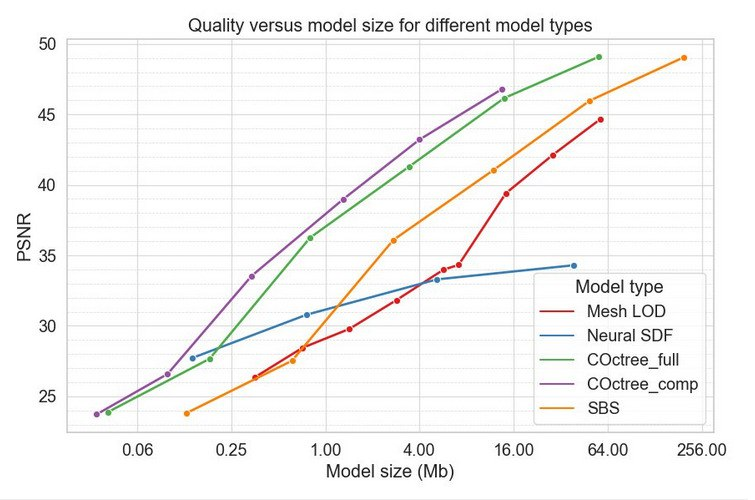
\includegraphics[width=0.5\textwidth]{example.jpg}
  \caption{Пример (заменю названия на "метод1", "метод2" и тд.)}
  \label{fig:example}
\end{figure}

\subsection{Освещение}
В данной работе используется один точечный источник света и простая модель освещения, так как задача - в первую очередь сравнить полученную каждым методом общую форму
объекта, не учитывая работу с материалами, множеством разных источников света, отражениями и т.д.

\medskip

Выбрана модель освещения Ламберта, работающая по следующему принципу:
\begin{enumerate}[leftmargin=4em]
	\item Если SDF(p) = 0, то p - точка на поверхности модели и нормаль к ней это - $n = \frac{\vec{l}}{\|l\|}, \ l = \frac{dSDF(p)}{dp}$.
	\item Цвет рассчитывается, как $c = max(0.1, \langle n, d \rangle)$, $d$ - вектор, направленный от точечного источника света к точке p.
\end{enumerate}

\begin{figure}[ht]
	\centering
	\begin{subfigure}[b]{0.3\textwidth}
			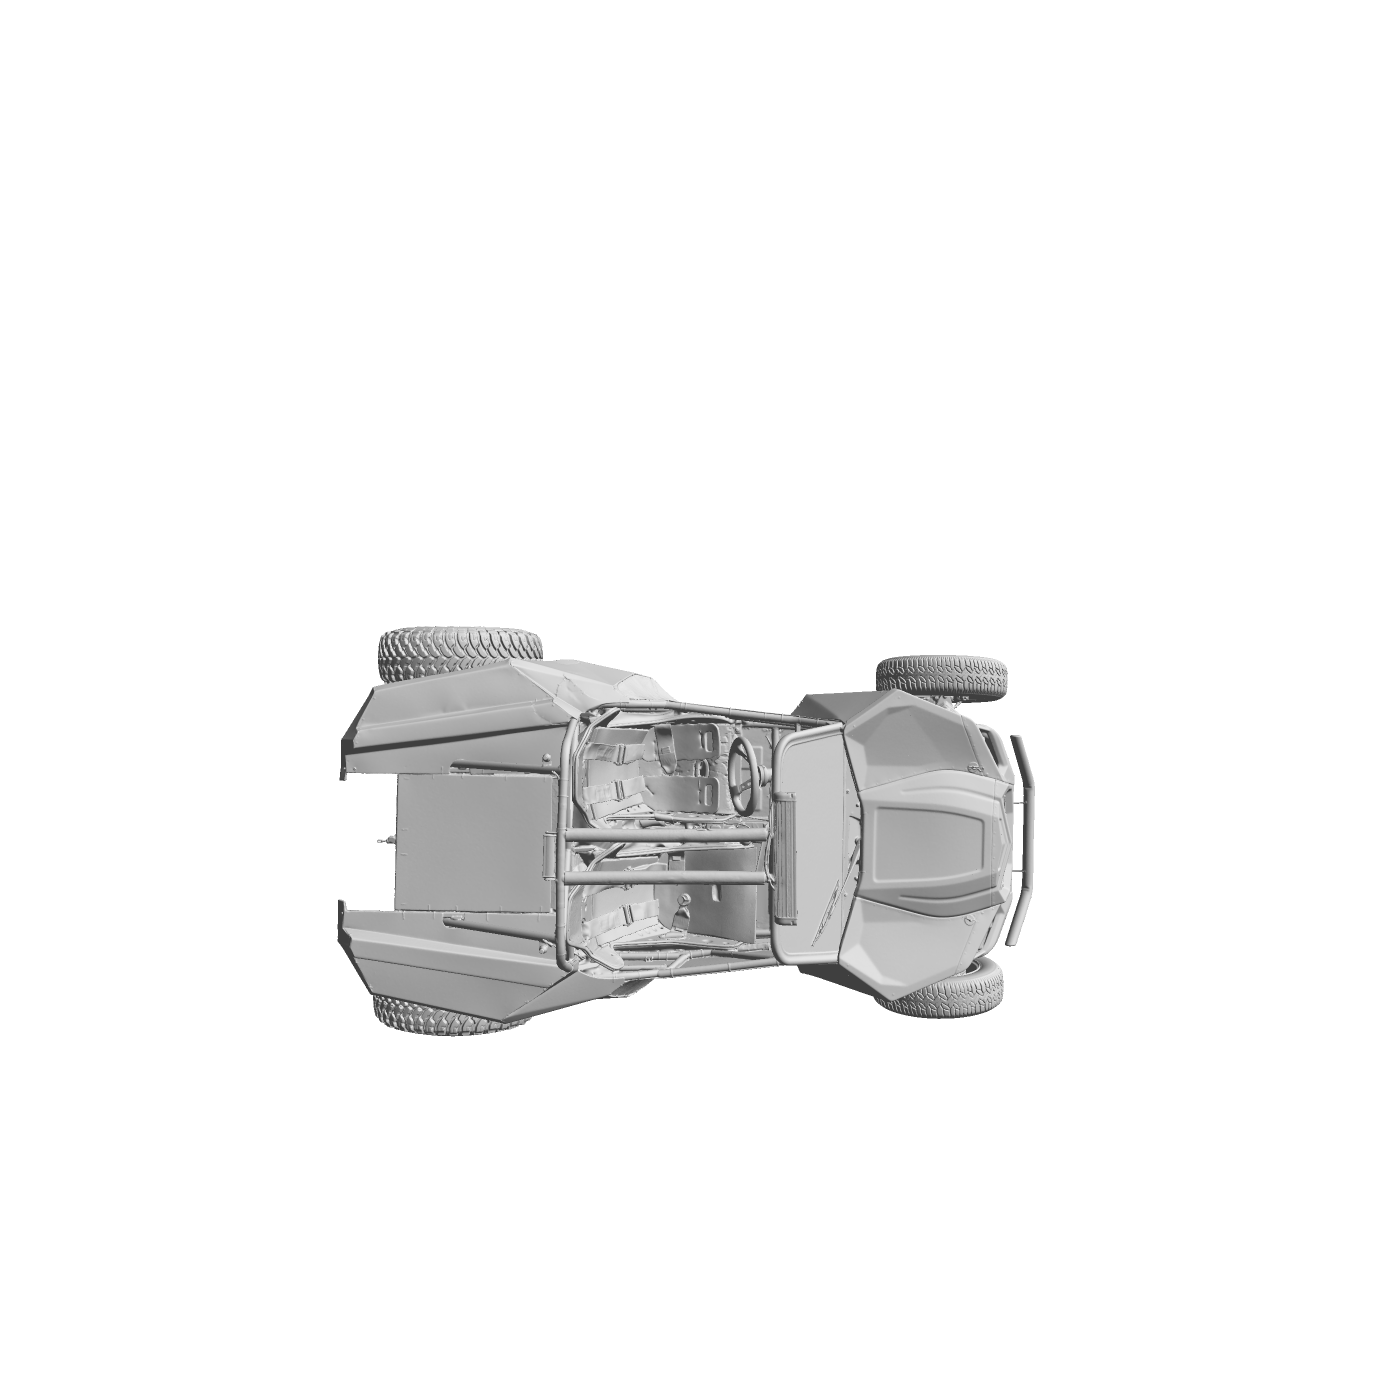
\includegraphics[width=\textwidth]{buggy.png}
			\caption{Buggy}
			\label{fig:img1}
	\end{subfigure}
	\hfill
	\begin{subfigure}[b]{0.3\textwidth}
			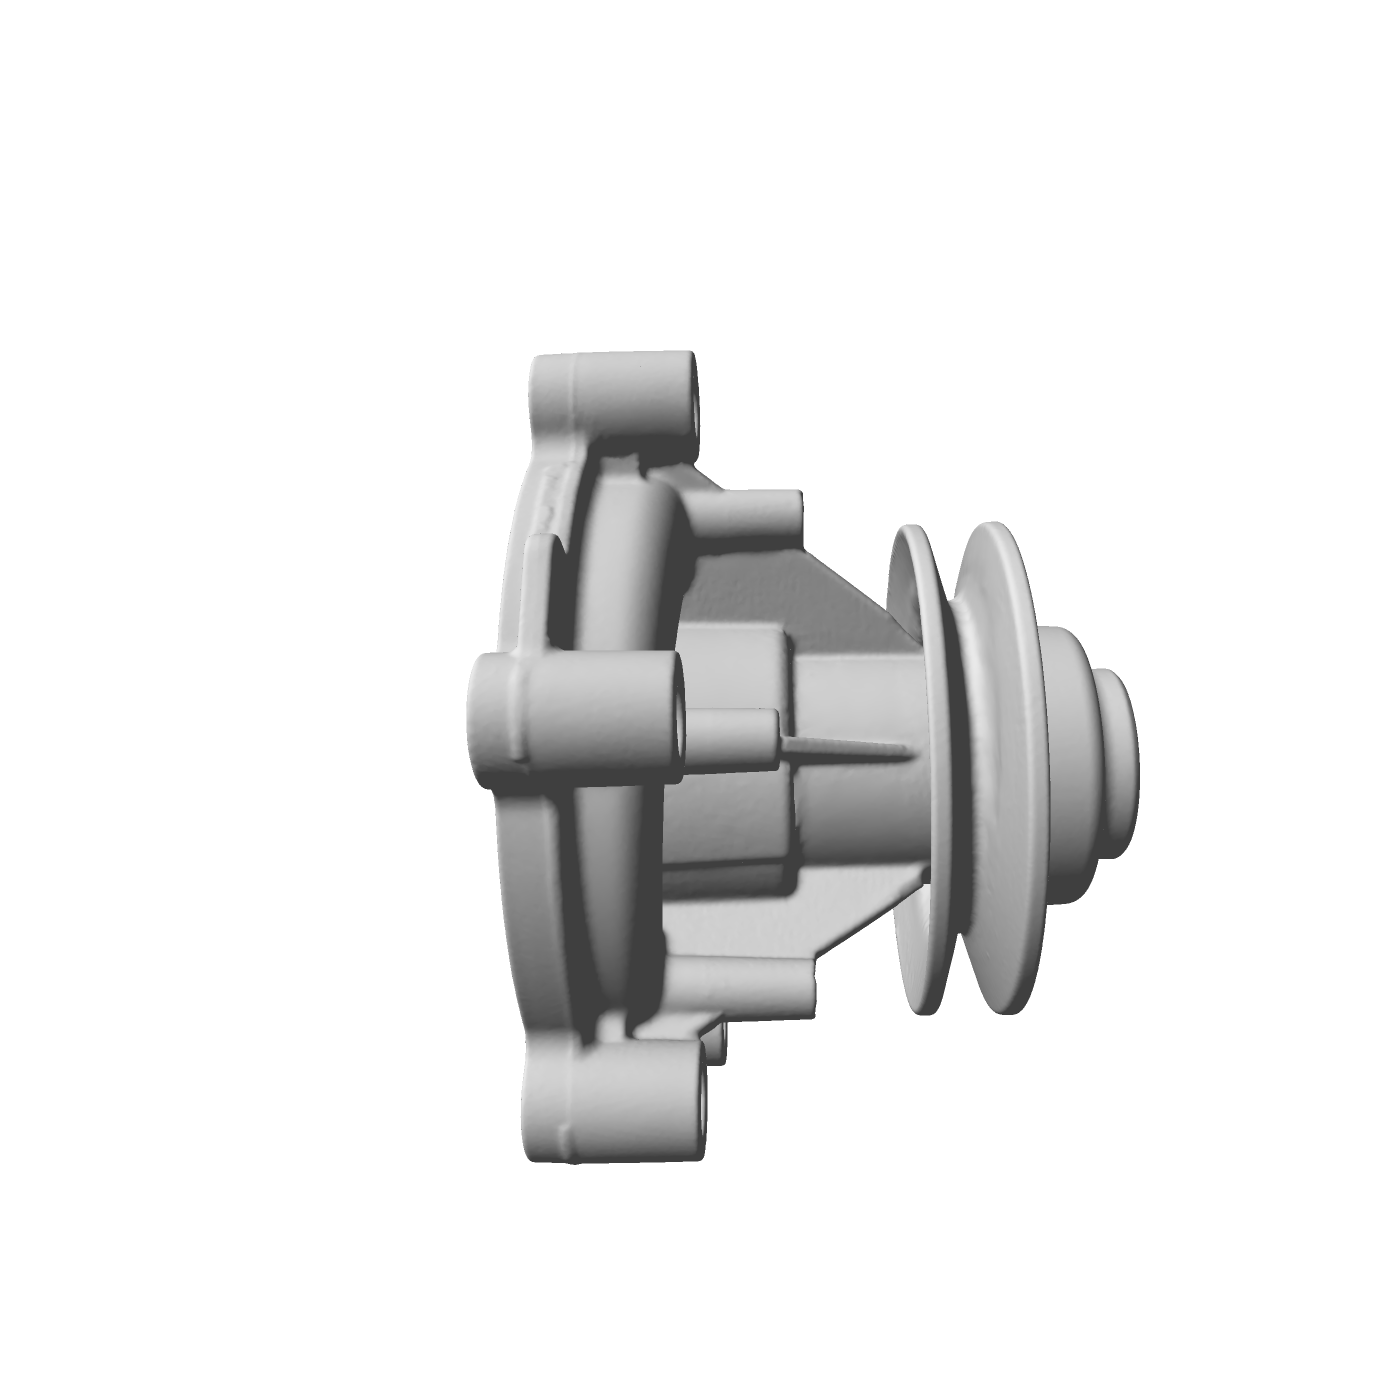
\includegraphics[width=\textwidth]{waterpump.png}
			\caption{Water Pump}
			\label{fig:img2}
	\end{subfigure}
	\hfill
	\begin{subfigure}[b]{0.3\textwidth}
			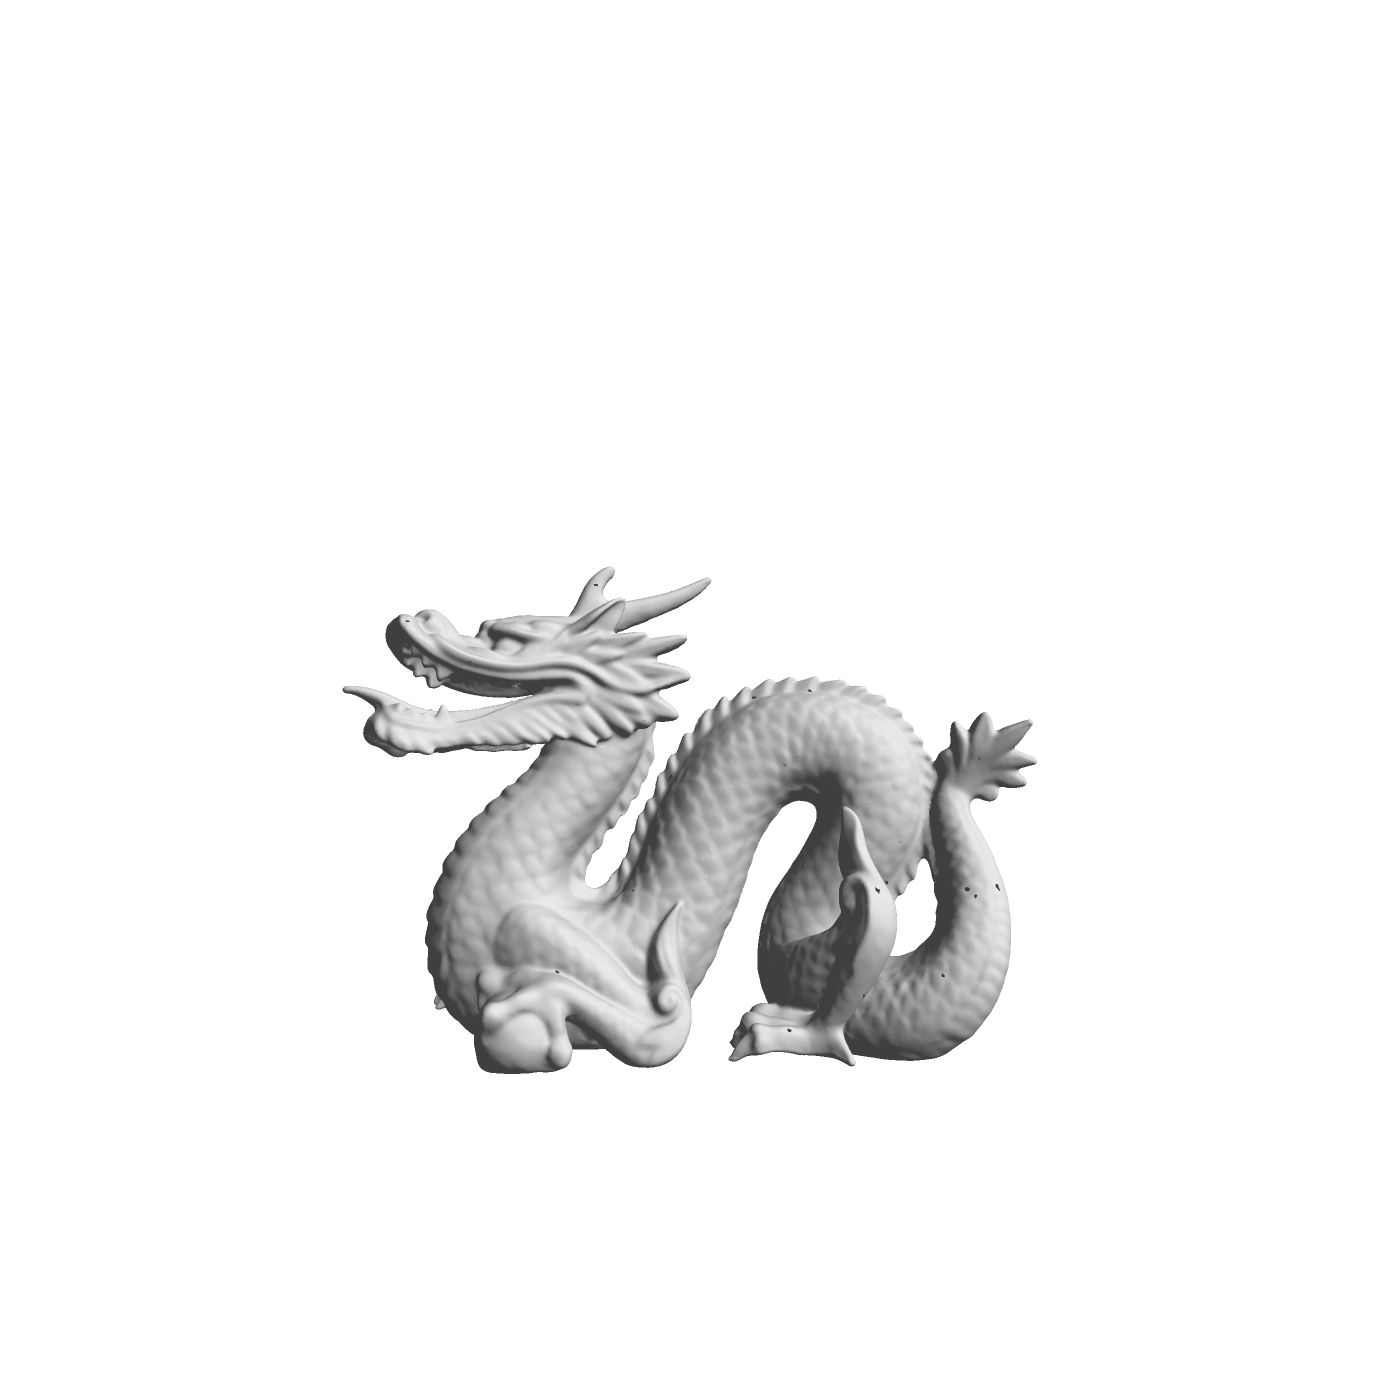
\includegraphics[width=\textwidth]{dragon.png}
			\caption{Dragon}
			\label{fig:img3}
	\end{subfigure}
	\caption{Примеры использования реализованного освещения}
	\label{fig:three-in-row}
\end{figure}

\newpage

\section{Практическая реализация}

\subsection{Структура бенчмарка}

В ходе проделанной работы был создан бенчмарк, который способен сравнивать, как методы, которые пользователь может реализовать сам, так и готовые решения, 
предоставляемые в виде готовых проектов. Есть возможность переносить написанные методы на графический ускоритель, используя средства Kernel Slicer [ссылка] для генерации кода для 
API Vulkan из С++ кода. Для такой трансформации кода написанные методы должны удовлетворять определенным тредованиям этого инструмента. 

Сцена может рисоваться 
как в режиме Мультирендера [ссылка на LiteRT], который использует стандартную трассировку и шагаюшую трассировку лучей для поиска пересечения с поверхностью, так и рендер систему 
HydraCore3 [ссылка], разрабатываемую в лаборатории компьютерной графики и мультимедиа факультета ВМК МГУ, которая способна рендерить реалистичные сцены
за счет использования трассировки пути. На рисунке 1 показана схема работы бенчмарка.

\begin{figure}[h]
  \centering
  \fbox{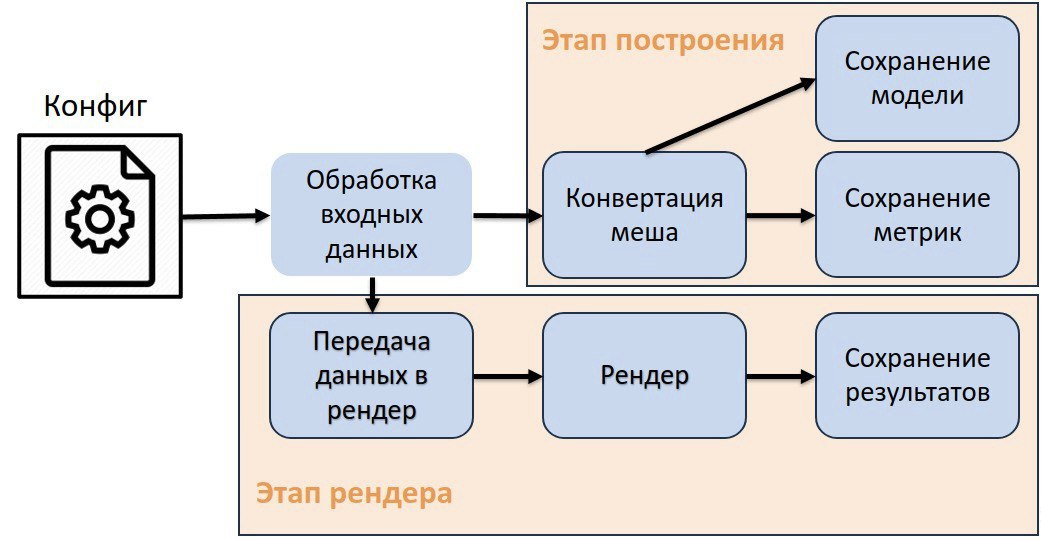
\includegraphics[width=1\linewidth]{bench_blocks.jpg}}
  \caption{Схема реализации сравнений методов между собой}
  \label{fig:my_label}
\end{figure}

\newpage

Работа бенчмарка идет в два этапа:
\begin{enumerate}
	\item Сборка каждым методом всех моделей с конкретными параметрами рендера. Полученные данные сохраняются в отдельные папки, откуда будут считываться во время рендера. Также записывается 
	время конвертации, размер и другие данные в специальный .csv файл.
	\item Во время рендера из каждой папки берутся данные и рендерятся. Результат сравнивается с референсным методом (по умолчанию это полигональная сетка) и сохраняется в .csv файл.
\end{enumerate}

\subsection{Возникшие проблемы}

Во время написания программы возниклом множество проблем. Их можно разделить на 4 группы:

\begin{enumerate}
	\item Методы, имеющие открытую программную реализацию, часто не имели нужных входных параметров. Например, позиция камеры, позиция источника света. В некоторых методах 
	модель нормализуется в куб $[-1, 1]^3$, а не $[-0.5, 0.5]^3$, что давало неверную картинку. Аналогичную проблему вызывали разные настройки камеры, потому что 
	данные о ней могли по-разному храниться и использоваться. Учитывая, что изначально метод мог вообще не принимать на вход информацию о ней, то приходилось 
	это исправлять. Другой проблемой было освещение, потому что, например, в нескольких методах используется модель физического освещения, а в других 
	обходятся обычным рассчетом мест затенения, поэтому приходилось убирать такую сложную модель освещения и заменять на более простую, чтобы полученные картинки 
	совпадали по теням и цвету. 
	\item Возникла проблема организации хранения данных, потому что очень много параметров, которые меняют выходной результат. Таким образом, на первом этапе 
	бенчмарк сохраняет в отдельную папку бинарный файл с моделью и .xml файл, который используется для её дальнейшей загрузки в выбранную систему рендера. На втором этапе создается 
	другая папка, которая будет содержать отрендеренные изображения. На этом шаге сначала рисуется эталонный метод, чтобы другие реализации могли сразу с ним 
	сравниваться. Все полученные результаты метрик записываются в третью папку. Выбранный подход позволяет получить на каждом этапе простую иерархию данных.
	\item При добавлении метода "Массово-параллельный рендеринг сложных неявных поверхностей замкнутой формы" (MPR) пришлось решать проблему, связанную с тем, 
	что его было не с чем сравнивать, потому что он рендерит конструктивную сплошную геометрию, представленную в виде дерева, а не полигональной сеткой. Для этого метода пришлось 
	реализовывать свое синтаксическое дерево, которое уже могло использоваться, как функция дистанции. Следовательно, появился способ сравнивать SDF методы c 
	методами, реализующими конструктивную сплошную геометрию. Такой подход позволяет использовать бенчмарк для более широкого класса методов, которые изначально 
	могут не иметь возможность сравнения с уже добавленными вариантами.
	\item Самая сложная возникшая задача - привести методы в сравнимый вид, потому что они все по-разному программно устроены и зависят от разных параметров, 
	оптимальный подбор которых дал бы объективные графики сравнения. Так как хотелось бы получить модели примерно одинакового веса, чтобы методы могли 
	честно соревноваться в скорости рендера и качестве полученных картинок.
\end{enumerate}

\newpage

\section{Эксперименты и результаты}

Графики size-psnr и таблички с изображениями, отсортированными по размеру модели, чтобы показать, как от увеличения размера меняется качество.

\subsection{Компромисс между памятью и качеством}

Разработанный метод приведения методы в сравнимый вид дал возможность графически визуализировать возможности каждой реализации.

\begin{figure}[ht]
  \centering
  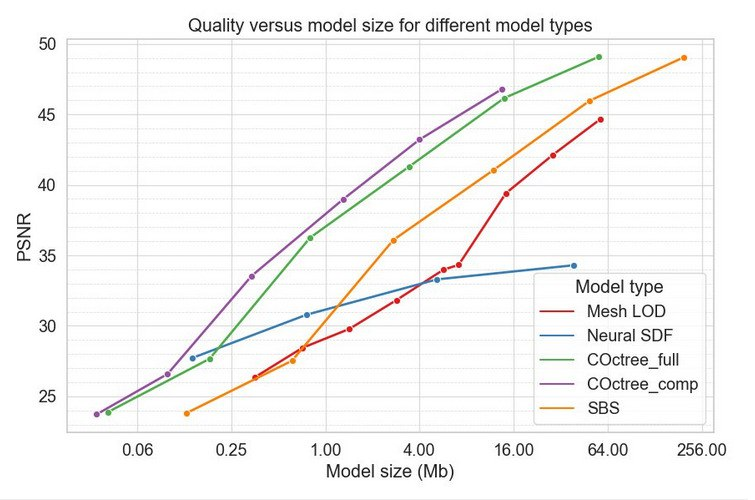
\includegraphics[width=0.5\textwidth]{example.jpg}
  \caption{Пример, пока что измерения считаются}
  \label{fig:example}
\end{figure}

\subsection{Выводы}

графики size-psnr с областями web, графика реального времени, кино фотореализм

таблица с баллами, которые каждый метод получил

вывод про то, для чего каждый метод лучше всего подходит

\newpage

\section{Заключение}

В ходе работы были получены следующие результаты:

\begin{itemize}
	\item Проведен обзор существующих работ по представлениям функций дистанции со знаком.
	\item Разработана методология сравнения методов.
	\item Полученна программная система для сравнительного анализа.
	\item Проведены экспериментальные сравнения выбранных представлений SDF.
	\item Проанализированны результаты и сделаны выводы.
\end{itemize}

\newpage

\section{Список литературы}

\end{document}
